\documentclass[c]{beamer}
\usepackage{color}
\definecolor{mythemecolor}{RGB}{168,0,0}
\setbeamercolor{structure}{fg=cyan!90!black}
\usepackage[frenchb]{babel}
%\usepackage[T1]{fontenc}
\usepackage[utf8]{inputenc}
\usepackage{tikz}
\usetikzlibrary{calc,trees,positioning,arrows,chains,shapes.geometric,decorations.pathreplacing,decorations.pathmorphing,shapes,matrix,shapes.symbols}
\tikzset{
    >=stealth',
    punktchain/.style={
      rectangle, 
      rounded corners, 
      draw=black, very thick,
      text width=10em, 
      minimum height=3em, 
      text centered, 
      on chain},
    line/.style={draw, thick, <-},
    element/.style={
      tape,
      top color=white,
      bottom color=blue!50!black!60!,
      minimum width=8em,
      draw=blue!40!black!90, very thick,
      text width=10em, 
      minimum height=3.5em, 
      text centered, 
      on chain},
    every join/.style={->, thick,shorten >=1pt},
    decoration={brace},
    tuborg/.style={decorate},
    tubnode/.style={midway, right=2pt},
}
%\usepackage{graphicx}

\title[Soutenance de Projet Industriel]{Implémentation du pipeline OpenHaRT sur la plateforme DAE}
\author{Julien BIDOLET \and Clément AUDAM \and Pierre P\'EZOT }
%\date{7 septembre 2013}
\institute{TELECOM Nancy}
\titlegraphic{
\includegraphics[width=2.5cm]{telecom_nancy.png}
\hspace{1cm}

\includegraphics[width=2.5cm]{loria.jpg}
}


\usetheme{Warsaw}
%\usecolortheme{spruce}

\addtobeamertemplate{footline}{\insertframenumber/\inserttotalframenumber}

\begin{document}


\begin{frame}
  \maketitle
\end{frame}

\begin{frame}
  \tableofcontents
\end{frame}
\section{Contexte}
\section{Gestion}
		    

\section{Travail réalisé}
\subsection{Analyse d'OpenHaRT}
\begin{frame}
\begin{columns}[c]
\begin{column}{.6\textwidth}
    \begin{block}{Analyse du pipeline}
        \begin{itemize}
            \item Analyse de la structure du pipeline
            \item Etude du format MADCAT
            \item Etude des métriques
        \end{itemize}
    \end{block}
    \begin{block}{Inconvénients du pipeline actuel}
        \begin{itemize}
            \item Installation complexe
            \item Utilisation peu intuitive
            \item La structure actuelle ne favorise pas les évolutions
        \end{itemize}
    \end{block}
\end{column}
\begin{column}{.4\textwidth}
\begin{figure}
\scalebox{.6}{
\begin{tikzpicture}
      [node distance=.8cm, start chain=going below,]
      \node[punktchain, join] (madcatIn) {Copie des fichiers d'entrée MADCAT};
      \node[punktchain, join] (algo)      {Exécution de l'algorithme};
      \node[punktchain,join] (metricGen) {Conversion de la sortie de l'algorithme en fichiers pour métriques};      
      \node (met1) [punktchain, join ]  {Exécution des métriques};     
      \node[punktchain, join,] (summary) {Bilan}; 
\end{tikzpicture}
}
\\Structure du pipeline
\end{figure}
\end{column}
\end{columns}
\end{frame}

\subsection{Etude de DAE}
\begin{frame}

\begin{block}{La plateforme DAE}
\begin{itemize}
\item Prise en main des services web.
\item Adaptation du format MADCAT au format de données DAE.
\item Visualisation des informations stockées sur l'interface web de la plateforme.
\end{itemize}
\end{block}
\begin{figure}
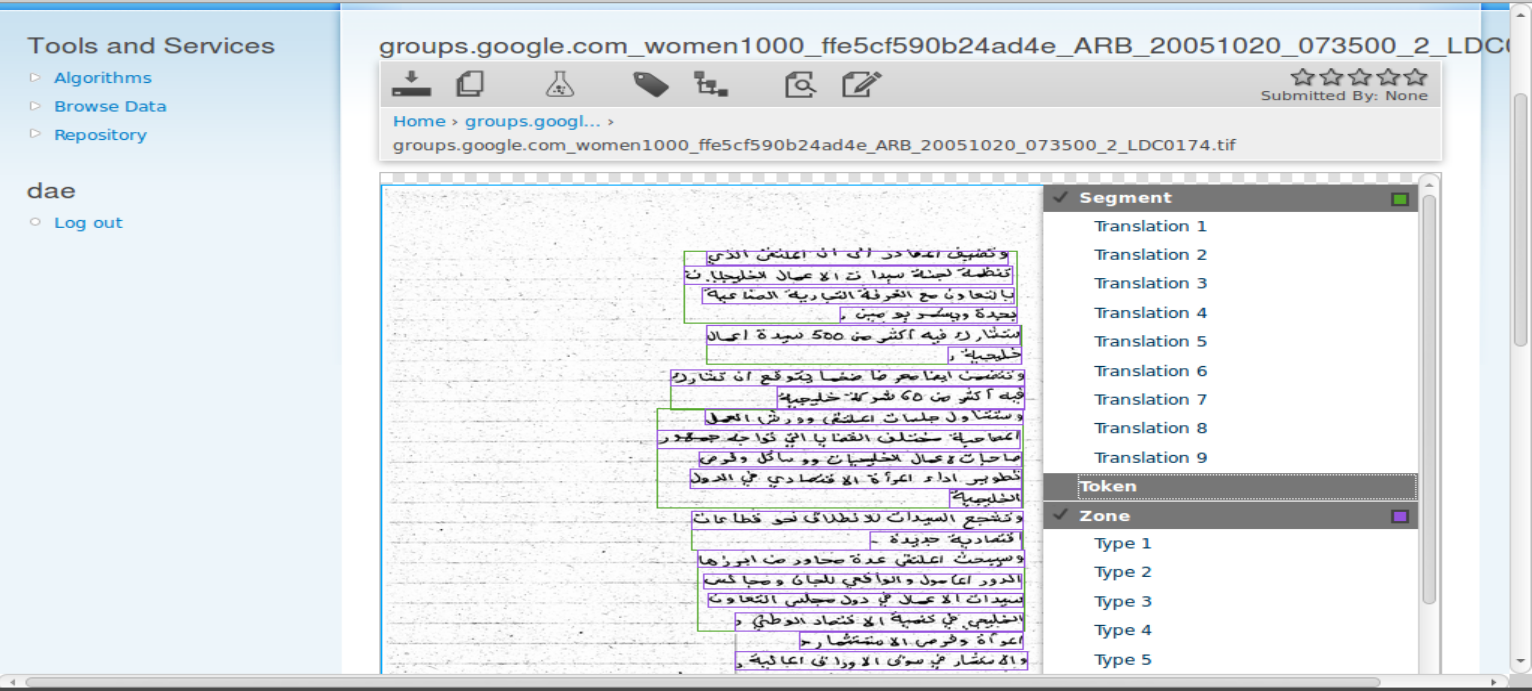
\includegraphics[scale=.1]{DAEElements}
\\Visualisation d'un document manuscrit arabe
\end{figure}

\end{frame}
\subsection{Implémentation du pipeline sur DAE}

\begin{frame}[t]

\begin{block}{Objectif}
        Implémenter le processus OpenHaRT dans un pipeline dont les briques de base sont des services web
\end{block}
\begin{columns}[c]
\begin{column}{.6\textwidth}
\begin{block}{Implémentation}
\begin{itemize}
    \item Ecriture des programmes d'accès à la base de données.
    \item Passage des différents programmes en services web.
    \item Chaînage des services web pour former le pipeline.
\end{itemize}
\end{block}
\end{column}
\begin{column}{.5\textwidth}
    \scalebox{.4}{
    \begin{tikzpicture}[node distance=.8cm,start chain=going below,]
        \node[punktchain, join] (madcatIn) {Génération du fichier d'entrée MADCAT};
        \node[punktchain] (algo)      {Exécution de l'algorithme};
        \draw[->,>=latex, thick, dashed] (madcatIn) -- (algo);
        \node[punktchain, join] (madcat2Db)      {Insertion des résultats dans la base de données}; 
        \node[punktchain] (metricGen) {Génération des fichiers d'entrée des métriques}; 
        \draw[->,>=latex, thick, dashed] (madcat2Db) -- (metricGen);
                                         
        \node (met1) [punktchain, join ]  {...};
        \begin{scope}[start branch=1]
            \node[punktchain, on chain = going left](met2) {Métrique 1};
        \end{scope}
        \begin{scope} [start branch=2]
            \node[punktchain, on chain= going right]  (met3)  {Métrique n};
        \end{scope}
        \node[punktchain, join,] (summary) {Bilan};
        \draw[->,>=latex, thick] (metricGen) -| (met3);
        \draw[->,>=latex, thick] (metricGen) -| (met2);
        \draw[->,>=latex, thick] (met2) |- (summary);
        \draw[->,>=latex, thick] (met3) |- (summary);
    \end{tikzpicture}
    }
        \centering
        \\Structure du nouveau pipeline
\end{column}
\end{columns}
\end{frame}
\subsection{Documentation}
\begin{frame}
    \begin{block}{Documentation}
        \begin{itemize}
            \item Rédaction d'une documentation technique la plus complète possible
            \item Réflexion sur les améliorations et évolutions possibles de notre travail
        \end{itemize}
    \end{block}
    \begin{block}{Améliorations et évolutions}
        \begin{itemize}
            \item Prise en compte de plusieurs utilisateurs.
            \item Stockage des caractères arabes.
            \item Implémentation des pipelines DIR et DTT.
            \item Optimisation des communications de données.
            \item Automatisation de l'ajout de services.
        \end{itemize}
    \end{block}
\end{frame}
\section{Conclusion}
\begin{frame}
  \begin{block}{Conclusion}
    \begin{itemize}
        \item Specifications and learning phases have been completed
        \item Starting implementation
        \item  We would like to thanks Bart Lamiroy and Jean-François Scheid for their help.
     \end{itemize}
  \end{block}
\end{frame}
\end{document}
